\chapter{Spazi a curvatura costante}\label{para.curvacost}
Nel precedente capitolo sulla cosmologia è stato mostrato come l'omogeneità e l'isotropia inducano sulle ipersuperfici di omogeneità una particolare forma del tensore di Riemann, eq. \ref{eq.riemann_curvatura_costante}, ed è stato detto che una varietà che abbia il Riemann che rispetti tale equazione sia detta a curvatura costante. Si è anche accennato alla catalogazione che posseggono gli spazi di dimensione $n$ con metrica di segnatura $n$, ovvero l'isometria con lo spazio iperbolico, euclideo e alla $n$-sfera a seconda del segno della costante $k$. Alla fine del capitolo è stata fornita una catalogazione analoga per gli spazi di metrica lorentziana, ovvero con lo spazio di Anti-de Sitter, di Minkowski e de Sitter, i quali dipendono invece dalla costante cosmologica.

In questo capitolo verranno affrontati nuovamente questi concetti in maniera più sistematica, mostrando per i vari spazi i principali sistemi di coordinate adottati.

\section{Spazio di Einstein}
Uno spazio a curvatura costante di dimensione $n$, ha il tensore di Riemann completamente determinato da:
\begin{equation*}
    R_{\mu\nu\rho\sigma} = \lambda ( g_{\nu\sigma}g_{\mu\rho}  - g_{\nu\rho}g_{\mu\sigma})
\end{equation*}
dove $\lambda= \textrm{cost.}$. Contraendo, seguono:
\begin{align*}
    R_{\nu\sigma} &= \lambda (n-1) g_{\nu\sigma} \\
    R &= \lambda n(n-1) \\
    G_{\nu\sigma} &= - \frac{1}{2}(n-1)(n-2) g_{\nu\sigma}
\end{align*}
Riprendendo le equazioni di Einstein, $G_{\nu\sigma} + \Lambda g_{\nu\sigma} = 0$, è possibile legare la costante di curvatura con la costante cosmologica:
\begin{equation*}
    \Lambda = \frac{(n-1)(n-2)}{2}\lambda = \frac{n-2}{2n}R
\end{equation*}

Si ricorda inoltre il teorema \ref{teo.killing} che determina che uno spazio a curvatura costante ha il numero massimo di vettori di Killing possibili.

\begin{definizione}
Una varietà che ha tensore di Einstein proporzionale alla metrica viene detto \textbf{spazio di Einstein}.
\end{definizione}
Alcuni testi matematici, vedi \cite{bruhat_manifolds}, riportano come definizione che il tensore di Ricci sia proporzionale alla metrica (del tutto equivalente).
Da questa definizione segue che:
\begin{equation*}
    \textrm{curvatura cost.} \implies \textrm{spazio di Einstein}
\end{equation*}
mentre in generale non è vero il viceversa, infatti lo spaziotempo di Schwarzschild ha $\Lambda = 0$, ma non è a curvatura costante. \'E però vero che in $n=3$ vale il viceversa, poiché in questo caso il tensore di Weyl, eq. \ref{eq.tensore_weyl}, è identicamente nullo e pertanto il tensore di Riemann dipende solamente dal tensore di Schouten secondo eq. \ref{eq.decomposizione_riemann_weyl}. A sua volta lo Schouten dipende dal Ricci e quindi dalla metrica, pertanto si ottiene uno spazio a curvatura costante. 

L'Universo di Einstein $\mathbb R \times S^3$ non è uno spazio di Einstein; una parte di esso è lo spazio di Minkowski che invece è spazio di Einstein con $\Lambda = 0$ (vedi pag. 122 di \cite{hawking}).
\section{Spazio di de Sitter}
Lo spazio di de Sitter è caratterizzato dal possedere $\Lambda > 0$. Esso viene determinato dall'immersione nello spazio di Minkowski $(d+1)$-dim.\footnote{Si esegue un procedimento analogo a quello per le metriche di $H^3$, $S^3$.} che chiamiamo $\mathbb{R}^{d+1}_1$, con coordinate $X^A$, $A = 0,1, \dots, d$, e metrica:
\begin{equation*}
    \eta_{AB} = diag(-1,1,\dots, 1)
\end{equation*}
\begin{equation*}
    ds^2 = - d(X^0)^2 + d(X^1)^2 + \dots + d(X^d)^2 
\end{equation*}

Chiamiamo lo spaziotempo di de Sitter $d$-dim. $dS_d$ corrispondente all'ipersuperficie:
\begin{equation*}
    \eta_{AB}X^A X^B = l^2
\end{equation*}
o esplicitamente:
\begin{equation*}
    -(X^0)^2 + (X^1)^2 + \dots + (X^d)^2 = l^2
\end{equation*}
per $X^0$ fissato, si hanno delle $(d-1)$-sfere di raggio $r = \sqrt{l^2 + (x^0)^2}$:
\begin{equation*}
    (X^1)^2 + \dots + (X^d)^2 = l^2 + (X^0)^2
\end{equation*}
pertanto lo spazio di de Sitter $dS_d$ sono delle $S^{d-1}$ a $X^0$ fissato che si contraggono ad un raggio minimo per poi espandersi, fig. \ref{fig.spazio_desitter}. La metrica su $dS_d$ è quella indotta da $\mathbb{R}^{d+1}_1$.
\'E uno spazio a curvatura costante positiva ed è quindi spazio di Einstein con tensore di Riemann:
\begin{equation*}
    R_{\mu\nu\rho\sigma} = \frac{1}{l^2}( g_{\nu\sigma}g_{\mu\rho}  - g_{\nu\rho}g_{\mu\sigma})
\end{equation*}

Il gruppo di isometrie per $dS_d$ è $O(d,1)$, in quanto sono le isometrie di $\mathbb{R}^{d+1}_1$ e quindi per la metrica indotta. Il gruppo ha il numero massimo di generatori $\frac{1}{2}d(d+1)$.

\begin{figure}
    \centering
    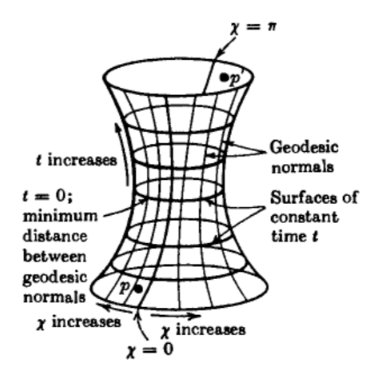
\includegraphics[scale=0.7]{immagini/spazio_desitter_embedding.png}
    \caption{Spazio di de Sitter $d$-dim. mostrato come immersione nello spazio di Minkowski $d+1$-dim.. Sono mostrate le coordinate globali che ricoprono l'intero iperboloide. Le superfici a $t = \textrm{cost.}$ sono $S^{d-1}$. }
    \label{fig.spazio_desitter}
\end{figure}
\subsection{Coordinate globali}
Ponendo $X^0 = l\sinh{\frac{\tau}{l}}$, si ottiene sostituendo:
\begin{equation*}
    (X^1)^2 + \dots + (X^d)^2 = l^2\cosh^2{\frac{\tau}{l}}
\end{equation*}
cioè delle $S^{d-1}$ con raggio $l\cosh{\frac{\tau}{l}}$. Si possono dunque introdurre delle coordinate sferiche nello spazio euclideo $\mathbb{R}^d$:
\begin{equation*}
    d(X^1)^2 + \dots + d(X^d)^2 = dr^2 + r^2d\Omega_{d-1}^2
\end{equation*}
dove $d\Omega_{d-1}^2$ è la metrica standard di $S^{d-1}$ di raggio 1. In questa maniera, usando il raggio precedente, si ottiene:
\begin{equation*}
        d(X^1)^2 + \dots + d(X^d)^2 = \sinh^2{\frac{\tau}{l}}dT^2 + l^2\cosh^2{\frac{\tau}{l}}d\Omega_{d-1}^2
\end{equation*}
e pertanto la metrica indotta su $dS_d$ nelle coordinate globali è:
\begin{equation}
    ds^2 = - d(X^0)^2 + d(X^1)^2 + \dots + d(X^d)^2 = - dT^2 + l^2\cosh^2{\frac{\tau}{l}}d\Omega_{d-1}^2
    \label{eq.desitter_globali}
\end{equation}
Sono coordinate che ricoprono l'intera varietà e la metrica è una forma di FLRW accelerante.

\subsection{Coordinate inflazionarie}
Utilizzando $(t, x^i)$ con $i= 1, \dots, d-1$ e $\bm{x}^2 = \sum_1^{d-1}x_i^2$, il sistema di coordinate è definito da:
\begin{align*}
    X^0 &= l\sinh\frac{t}{l} + \frac{\bm{x}^2}{2l}e^{t/l} \\
    X^i &= x^i e^{t/l} \\
    X^d &= l\cosh\frac{t}{l} - \frac{\bm{x}^2}{2l}e^{t/l}
\end{align*}
La metrica indotta risulta:
\begin{equation}
    ds^2 = \eta_{AB}dX^A dX^B = -dt^2 + e^{2t/l}d\bm{x}^2
    \label{eq.desitter_inflazionarie}
\end{equation}
dove $d\bm{x}^2$ è la metrica piatta $d-1$-dim..
Questa metrica è una forma di FLRW che ha le slice spaziali piatte, a coprire metà dello spazio $dS_d$.
\subsection{Coordinate statiche}
Le coordinate sono definite da:
\begin{equation*}
    (X^0)^2 - (X^d)^2 = r^2 - l^2
\end{equation*}
così che:
\begin{equation*}
    (X^1)^2 + \dots + (X^{d-1})^2 = r^2
\end{equation*}
corrispondente ad $S^{d-2}$. L'iperbole di $X^0$, $X^d$ può essere parametrizzata secondo:
\begin{align*}
    X^0 &= \sqrt{l^2 - r^2}\sinh \frac{t}{l} \\
    X^d &= \sqrt{l^2 - r^2}\cosh \frac{t}{l}
\end{align*}
con differenziali:
\begin{align*}
    dX^0 = -\frac{r}{\sqrt{l^2-r^2}}\sinh\frac{t}{l}dr &+ \frac{\sqrt{l^2-r^2}}{l}\cosh\frac{t}{l}dt \\
    dX^d = -\frac{r}{\sqrt{l^2-r^2}}\cosh\frac{t}{l}dr &+ \frac{\sqrt{l^2-r^2}}{l}\sinh\frac{t}{l}dt \\
    d(X^1)^2 + \dots + d(X^{d-1})^2 &= dr^2 + r^2 d\Omega_{d-2}^2
\end{align*}
La metrica indotta su $dS_d$ risulta:
\begin{equation}
    ds^2 = \eta_{AB}dX^A dX^B = - \left( 1 - \frac{r^2}{l^2} \right)dt^2 + \left(1 - \frac{r^2}{l^2}\right)^{-1}dr^2 + r^2 d\Omega_{d-2}^2
    \label{eq.metrica_desitter_statica}
\end{equation}

Questa metrica risulta simili a quella di Schwarzschild e presenta una singolarità delle coordinate in $r=l$ chiamata \textbf{orizzonte cosmologico}. Può solamente essere delle coordinate visto che negli altri sistemi di coordinate -- quello globale per primo -- non è presente.
\section{Spazio di Anti-de Sitter}
Consideriamo lo spazio $\mathbb{R}^{d+1}_2$ con coordinate $X^A$ dove $A = 0,\dots, d$ e metrica:
\begin{equation*}
    \eta_{AB} = diag(-1,1,\dots,1,-1)
\end{equation*}
Lo spaziotempo di Anti-de Sitter $AdS_d$ di dimensione $d$ è l'ipersuperficie:
\begin{equation*}
    \eta_{AB}X^A X^B = - l^2
\end{equation*}
Come gruppo di isometrie ha $O(d-1,2)$; il numero di generatori è massimo e pertanto è a curvatura costante (negativa).  La metrica indotta su $AdS_d$ ha il tensore di Riemann:
\begin{equation*}
    R_{\mu\nu\rho\sigma} = -\frac{1}{l^2}(g_{\nu\sigma}g_{\mu\rho} - g_{\nu\rho}g_{\mu\sigma})
\end{equation*}

Possiamo mostrare, ad esempio, $AdS_2$:
\begin{equation*}
    -(X^0)^2 + (X^1)^2 - (X^2)^2 = - l^2
\end{equation*}
dove per $X^1$ fissato si ottengono dei cerchi:
\begin{equation*}
       (X^0)^2 +  (X^2)^2 =  l^2 + (X^1)^2 
\end{equation*}
e lo spazio ha la forma mostrata in fig. \ref{fig.spazio_antidesitter}.
\begin{figure}
    \centering
    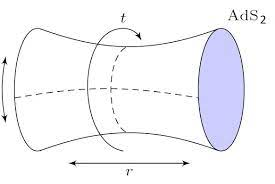
\includegraphics[scale=0.8]{immagini/spazio_antidesitter.jpeg}
    \caption{Topologia dello spazio $AdS_2$}
    \label{fig.spazio_antidesitter}
\end{figure}
\subsection{Coordinate globali}
Le coordinate globali su $AdS_d$ sono definite da:
\begin{equation*}
    (X^0)^2 + (X^d)^2 = r^2 + l^2 
\end{equation*}
dove:
\begin{equation*}
    (X^1)^2 + \dots + (X^{d-1})^2 = r^2
\end{equation*}
sono delle $S^{d-2}$ di raggio $r$. Il cerchio di $X^0$, $X^d$ può essere parametrizzato secondo:
\begin{align*}
    X^0 &= \sqrt{l^2 + r^2} \sin \frac{t}{l} \\
    X^d &= \sqrt{l^2 + r^2} \cos \frac{t}{l}
\end{align*}
La metrica indotta diventa:
\begin{equation}
    ds^2 = \eta_{AB}dX^a dX^B = - \left( 1 + \frac{r^2}{l^2}\right)dt^2 + \left( 1 + \frac{r^2}{l^2}\right)^{-1}dr^2 + r^2 d\Omega_{d-2}^2
    \label{eq.metrica_ads_statica}
\end{equation}
Questa metrica è simile alla metrica statica di $dS_d$, tuttavia non presenta più la singolarità per $r\rightarrow l$. \'E definita globalmente. Alcune volte questa metrica viene riscritta con il cambio di coordinate $r \mapsto l\sinh r$:
\begin{equation}
    ds^2 = -\cosh^2r dt^2 + l^2dr^2 + l^2\cosh^2r d\Omega_{d-2}^2
\end{equation}
\subsection{Coordinate di Poincarè}
Definendo le coordinate $(z, x^i,t)$ con $i = 1,\dots, d-2$ e $\bm{x}^2 = \sum (x^i)^2$,  legate secondo:
\begin{align*}
    X^0 &= \frac{z^2 + l^2 + \bm{x}^2 - t^2}{2z} \\
    X^i &= \frac{l}{z}x^i \\
    X^{d-1} &=  \frac{z^2 - l^2 + \bm{x}^2 - t^2}{2z} \\
    X^d &= \frac{l}{z}t
\end{align*}
La metrica indotta su $AdS_d$ diventa:
\begin{equation*}
    ds^2 = \eta_{AB}dX^A dX^B = \frac{l^2}{z^2}(- dt^2 + dz^2 + d\bm{x}^2)
\end{equation*}
Questa metrica è conformemente piatta.

Risulta utile mostrare il caso delle coordinate di Poincarè per $AdS_2$:
\begin{equation*}
    ds^2 = \frac{l^2}{z^2}(-dt^2 + dz^2)
\end{equation*}
se si esegue $z= \frac{l^2}{\rho}$ e si sostituisce si ottiene:
\begin{equation*}
    ds^2 = - \frac{\rho^2}{l^2}dt^2 + \frac{l^2}{\rho^2}d\rho^2
\end{equation*}
\subsection{Coordinate in forma FLRW}
Si esegue il cambio di coordinate secondo:
\begin{align*}
    X^0 &= l\sin\frac{\tau}{l} \\
    X^i &= l\cos\frac{\tau}{l}\sinh\rho x^i \\
    X^d &= l\cos\frac{\tau}{l}\cosh\rho
\end{align*}
così $\bm{x}^2 = \sum_1^{d-1} x^i = 1$ ovvero una $S^{d-2}$ di raggio 1. La metrica indotta su $AdS_d$ risulta:
\begin{equation*}
    ds^2 = - dT^2 + l^2\cos^2\frac{\tau}{l}(d\rho^2 + \sinh^2\rho d\Omega_{d-2}^2)
\end{equation*}
Le slice spaziali sono gli spazi iperbolici $H^{d-1}$. Osserviamo che si può avere in questa forma un \virgolette{big crunch} per $\tau/l = \frac{\pi}{2}$, ma è un artefatto delle coordinate poiché non viene osservato in quelle globali.
\section{Buchi neri immersi in AdS/dS}
Consideriamo la metrica:
\begin{equation}
    ds^2 = - \left( 1 - \frac{m}{r^{d-3}} + \frac{r^2}{l^2} \right)dt^2 + \left( 1 - \frac{m}{r^{d-3}} + \frac{r^2}{l^2} \right)^{-1}dr^2 + r^2d\Omega_{d-2}^2
    \label{eq.bh_in_ads}
\end{equation}
dove $m$ è un parametro di massa. Questa soluzione rappresenta uno spazio di Einstein senza però essere a curvatura costante. Si notano i casi limite:
\begin{itemize}
    \item $m=0 \implies AdS_d$
    \item $l\rightarrow + \infty \implies $ Schwarzschild in $d$-dim., detta  anche soluzione di \textbf{Schwarschild-Tangherlini}
\end{itemize}
I buchi neri immersi in $dS_d$ possono essere ottenuti dalla precedente metrica eseguendo la trasformazione $\frac{r^2}{l^2}\rightarrow - \frac{r^2}{l^2}$.

La metrica di eq. \ref{eq.bh_in_ads} può essere generalizzata, similmente a quanto effettuato per dedurre la soluzione di Schwarzschild, secondo:
\begin{equation}
    ds^2 = -\left( k - \frac{m}{r^{d-3}} + \frac{r^2}{l^2}  \right)dt^2 + \left( k - \frac{m}{r^{d-3}} + \frac{r^2}{l^2} \right)^{-1}dr^2 + r^2d\Sigma_{k, d-2}^2
    \label{eq.bhs_topolog_generaliz}
\end{equation}
dove $k = -1,0,1$ e $d\Sigma_{k,d-2}^2$ è, a seconda del valore $k$, la metrica su $H^{d-2}$, $\mathbb{E}^{d-2}, $$S^{d-2}$.
Questa generalizzazione risolve le equazioni di Einstein:
\begin{equation*}
    G_{\mu\nu} + \Lambda g_{\mu\nu} = 0
\end{equation*}
e ha orizzonte degli eventi nello zero più grande di $ k- \frac{m}{r^{d-3}} + \frac{r^2}{l^2} $. Nei casi $k=0, -1$ l'orizzonte non è compatto, ma può essere eseguita la compattificazione.
\begin{esempio}
Si considera $d = 4$ e $k=0$ in eq. \ref{eq.bhs_topolog_generaliz}. La compattificazione  viene eseguita tramite le coordinate di Hopf e l'immersione in $S^3$ che trasforma la metrica in:
\begin{equation*}
    ds^2 = d\alpha^2 + \cos^2\alpha d\phi^2 + \sin^2 \alpha d\psi^2
\end{equation*}
dove $\alpha \in [0,\frac{\pi}{2}]$, $ \phi \in [0,2\pi]$, $\psi \in [0, 2\pi]$.  Le sottovarietà a $\alpha = \textrm{cost.}$ sono un toro di Clifford, o toro piatto. Si parla infatti di buchi neri topologici in quanto posseggono un orizzonte dalla topologia non banale.
\end{esempio}